% https://www.tandfonline.com/toc/goms20/current
\documentclass[]{interact}

\usepackage[caption=false]{subfig}% Support for small, `sub' figures and tables
%\usepackage[nolists,tablesfirst]{endfloat}% To `separate' figures and tables from text if required

%\usepackage[doublespacing]{setspace}% To produce a `double spaced' document if required
%\setlength\parindent{24pt}% To increase paragraph indentation when line spacing is doubled
%\setlength\bibindent{2em}% To increase hanging indent in bibliography when line spacing is doubled

\usepackage[numbers,sort&compress]{natbib}% Citation support using natbib.sty
\bibpunct[, ]{[}{]}{,}{n}{,}{,}% Citation support using natbib.sty
\renewcommand\bibfont{\fontsize{10}{12}\selectfont}% Bibliography support using natbib.sty

\usepackage{enumitem}
\usepackage{amssymb,amsmath}
\usepackage{graphicx}
\usepackage{tikz}
\usetikzlibrary{patterns}
\usepackage{theoremref}

\graphicspath{{media/}}

\theoremstyle{plain}% Theorem-like structures provided by amsthm.sty
\newtheorem{theorem}{Theorem}[section]
\newtheorem{lemma}[theorem]{Lemma}
\newtheorem{corollary}[theorem]{Corollary}
\newtheorem{proposition}[theorem]{Proposition}

\theoremstyle{definition}
\newtheorem{definition}[theorem]{Definition}
\newtheorem{example}[theorem]{Example}

\theoremstyle{remark}
\newtheorem{remark}{Remark}
\newtheorem{notation}{Notation}
\newtheorem{condition}{Condition}

\begin{document}

\title{A novel algorithm for construction of the shortest path
between a finite set of nonintersecting contours on the plane}

\author{
\name{
  A.~A. Petunin\textsuperscript{a}\textsuperscript{b},
  E.~G. Polishchuk\textsuperscript{a}
  and
  S.~S. Ukolov\textsuperscript{a}\thanks{CONTACT S.~S. Ukolov. Email: s.s.ukolov@urfu.ru}}
\affil{
  \textsuperscript{a}Ural Federal University, Yekaterinburg, Russia
  \textsuperscript{b}Institute of Mathematics and Mechanics, UBr RAS, Yekaterinburg, Russia
}}

\maketitle

\begin{abstract}
The article discusses one of the optimization problems
that arise when modeling the tool path for CNC sheet metal
cutting machines for the case when the boundary contours
of the parts are defined by polygons and the pierce points
are located on the boundary contours.
Only closed-loop cutting is used,
i.e. Continuous Cutting Problem (CCP),
hence
the task of minimizing the length of the tool path
is reduced to the problem of finding the minimum air move length,
which is shown to be equivalent to the problem of finding
the shortest polyline with vertices on disjoint contours in the plane,
while these contours do not contain internal contours.
An algorithm for constructing minimal length broken line
for a fixed order of cutting contours is described
and is proved to provide local minimum.
Sufficient conditions for this minimum to be global are given.
Heuristic algorithm is suggested for finding the optimal order for cutting contours.
The results of a computational experiment
and a comparison of the results with an exact solution for the GTSP problem are presented.

\end{abstract}

\begin{keywords}
  Continuous optimization;
  Discrete optimization;
  Fermat principle;
  Variable Neighborhood Search
\end{keywords}

\section{Introduction}

A number of optimization problems arise
during development of control programs for CNC sheet cutting machines.
One of them is
the task of minimizing the tool air move,
which in some special cases can be reduced
to the problem of finding the shortest polyline
with vertices on flat contours.
Contours are interpreted as the boundaries of flat parts.
The location of the contours on the plane is determined
during the solution of the ``nesting'' problem.
Both tasks are generally NP-hard.

In its turn,
the task of minimizing tool air move
is a subtask of another optimization problem --
the task of optimizing the tool path when cutting flat parts.
Its exact solution cannot be obtained for problems
that actually arise in production
(for hundreds of parts / contours) in a reasonable time,
therefore,
various heuristics are typically applied
to get solutions of acceptable quality.
At the same time, the issues of developing algorithms
that provide optimal solutions for some problem cases,
as well as evaluating the quality of their solutions
in comparison with the optimal solution,
remain unresolved and are of significant scientific interest.

The general problem of optimizing the tool path
when cutting 2D objects on CNC machines,
which consists in minimizing cutting time and cost,
includes a whole range of different optimization tasks.
A classification of such problems
can be found
in \cite{bi01,bi02,bi03}.

\begin{itemize}
  \item
  Continuous Cutting Problem (CCP): each closed contour (that bounds a part)
  is cut out entirely by one movement of the torch,
  but cutting can start from any point (and finishes at the same point).

  \item
  Generalized Traveling Salesman Problem (GTSP):
  cutting can start only at one of the predefined points on the contour,
  the contour must be cut entirely.

  \item
  Endpoint Cutting Problem (ECP):
  cutting can start only at one of the predefined points on the contour,
  and the contour can be cut in several approaches, in parts.

  \item
  Segment Continuous Cutting Problem (SCCP):
  the notion of a cutting segment is introduced,
  which is a generalization of a contour;
  it can be either a part of a contour
  or a combination of several contours or their parts.
  Each segment is cut out entirely, thus
  $ CCP \subset SCCP$.

  \item
  Generalized Segment Continuous Cutting Problem (GSCCP):
  segment cutting (SCCP),
  but the selection of segments is not fixed in advance,
  but is subject to optimization

  \item
  Intermittent Cutting Problem (ICP):
  the most general cutting problem described in the literature,
  when contours can be cut in parts,
  in several approaches,
  and cutting can begin at any point in the contour.
\end{itemize}

Tool path optimization problems
in practice often reduce to discrete optimization problems
by discretizing the contours to be cut with a certain step
$\varepsilon$,
that is, they reduce to ECP
\cite{bi04,bi05,bi06}
or its special case, GTSP
\cite{bi07,bi08,bi09,bi10}.
CCP can also be reduced to GTSP.
In this case, however,
the total error in the air move length reaches
$N \cdot \varepsilon$,
where $N$ is the number of contours.
To guarantee the accuracy of the result of
$\delta$,
it is necessary to choose a small
$\varepsilon \approx \delta / N$,
so the total number of points on the contour grows
(as $O (N)$)
and the exhaustive search becomes exponential.
Nevertheless, such problems can be successfully solved,
for example, by the dynamic programming method,
for small
$N \approx 30$ even precisely
(see, in particular \cite{bi15}).

Tool path routing without using discretization (CCP)
is further considered in this paper.
The publications on this subject
are rare.
\cite{bi11,bi12}
can be noted,
where
heuristic algorithms are proposed.

\subsection{Technological constraints}

The need to execute the tool path on a
CNC sheet cutting machine imposes
a number of technological limitations on it.

The so-called ``precedence constraint''
is by far most popular in the literature.
It is caused by the fact that after cutting a closed contour,
its interior is usually not held by anything
and can freely shift, rotate and even fall.
For this reason,
the internal contours of parts must be cut
before the external contours containing them,
and parts located in the holes of large parts even earlier.

Finally, most cutting technologies require
that the cutting not be carried out strictly along the contour,
but with some indentation.
This shift can be performed both during the solution of the routing problem,
and after -- at the stage of generating the control program for the CNC cutting machine
or even by the machine itself during the cutting process.
In addition, the pierce point (tool switch-on point)
should generally be located even further
from the contour to avoid part damage.
However, this work completely ignores this requirement.
Thus, it is further assumed that the tool moves exactly
along the contour of the part
and the pierce point is located directly on the contour
(as well as the switch-off point of the tool).

\section{Continuous Cutting Problem}

Consider the Euclidean plane
$\mathbb R ^ 2$
and its region $B$ bounded by a closed contour
(rectangle in most cases),
which is a model of the sheet material to be cut.
Let $N$ pairwise disjoint flat contours
$\{C_1, C_2, ... C_N\}$
be given inside $B$, bounding $n$ parts
$\{A_1, A_2 ... A_n\}$.
A part can be limited by either one contour or several
(external and internal holes),
so that in general
$n \le N$.

The contours
$C_i$
can have an arbitrary shape,
but we will only consider the case
when they consist of (a finite number)
segments of lines and arcs of circles,
which is determined by the existing technological equipment.
In case when the contours consist only of line segments,
the continuous cutting problem
is reduced to one of the variants of the
Touring Polygon Problem (TPP),
see \cite{bi13}.

Further, two points are set in region $B$ (usually at its boundary),
we denote them as
$M_0$, $M_{N + 1}$
(almost always $M_0 = M_{N + 1}$),
which represent the beginning and end of the cutting route.

Continuous Cutting Problem is to find:
\begin{enumerate}
\item $N$ pierce points $M_i \in C_i, i \in \overline{1, N}$
\item Contour $C_i$ traversal order, i.e. permutations of $N$ elements $I = (i_1, i_2, ... i_N)$
\end{enumerate}

The result of solving the problem will be the route
$\{M_0, M_{i_1}, M_{i_2}, \dots M_{i_N}, M_{N + 1}\}$.
The objective function in this case is greatly simplified
in comparison with the general cutting problem
and is reduced to minimizing the air move length.

\begin{equation}
  \mathcal{L} = \sum_{j=0}^N|M_{i_j}M_{i_{j+1}}|
  \label{air-move-length}
\end{equation}
$$
\mathcal{L} \to \min
$$

Where, for simplicity, we introduce the notation
$M_{i_0} = M_0$,
$M_{i_{N + 1}} = M_{N + 1}$.

In addition,
we will solve the optimization problem
with an additional constraint,
the so-called ``precedence constraint''.
Although the contours $C_i$
do not intersect,
they can be nested into each other, i.e.,
$\tilde{C_a} ̃\subset \tilde{C_b}$,
where
$\tilde{C_a}$
denotes a 2-dimensional figure bounded by the contour
$C_a$
(in the more familiar notation
$C_a = \partial \tilde{C_a}$).
In the general tool path routing problem,
this can be caused by two different circumstances
(holes in parts and
placement of smaller parts
in holes larger to save material),
but in this case
these options are processed the same way.

If one contour is located inside another,
then the nested contour must be cut out
(visited)
earlier than the outer one:
$\tilde{C_a} ̃\subset \tilde{C_b} ̃\Rightarrow i_a < i_b$
in the permutation
$I = (i_1, i_2, ... i_N)$.
Thus, not all permutation of the contours are feasible.

\section{Algorithm to solve Continuous Cutting Problem}

The proposed solution algorithm
consists of several stages,
naturally associated with the nature of the problem being solved.

\subsection{Removal of external contours}

To automatically comply with the precedence constraint,
the first step removes all contours containing nested ones,
that is, only contours remain that satisfy the condition:
$$
\{C_i | \forall j \ne i: C_j \cap \tilde{C_i} = \varnothing \}
$$
This generally leads to a reduction
(in some cases significant)
of the size of the problem
(from $N$ to some $N'$),
and thus reduces the calculation time
in the second and especially the third stage.

\subsection{Continuous optimization}

At this stage,
we assume the bypass sequence
$I = (i_1, i_2, ... i_N)$
given and look for the coordinates of the pierce points
in each contour
$M_i \in C_i$,
minimizing the total air move length (\ref{air-move-length}).
To do this, the initial positions of the points are somehow selected
(randomly, for instance)
and the position of each pierce point $M_i$
changes under the assumption that others are fixed:
$\mathcal{L}(M_i) \to \min$.
Most terms in the objective function
(\ref{air-move-length})
are constant, therefore it simplifies to
$$
|M_{i-1}M_i|+|M_iM_{i+1}| \to \min_{M_i \in C_i}
$$

Moreover,
if the points
$M_{i-1}$,
$M_{i + 1}$
are located on opposite sides of the segment of the contour
$C_i$,
then the optimal position of the
pierce point $M_i$ is the intersection with the segment:
$M_i = M_{i-1} M_{i + 1} \cap C_i$
(if such an intersection exists;
otherwise,
the solution will be one of the ends of the segment).
If the points are located on one side of the segment,
then the solution can also be easily found using the
\textit{Fermat principle},
generating the famous rule
``the angle of incidence is angle of reflection''
(or again one of the ends of the segment),
see fig. \ref{fermat}.

\begin{figure}
  \begin{center}
  \tikz[rotate=27,scale=1.3]{
      \draw[thick]
          (0, 0) coordinate(zero) -- (5, 0) coordinate(future) node[right] {$C_i$};
      \fill[black]
          (1.5, 0) circle(0.1) coordinate(middle) node[below right]  {$M_i$}
          (1, 1) circle(0.1) coordinate(from) node[above left] {$M_{i-1}$} ++(-1.5,0) node[above] {$C_{i-1}$}
          (4.5, 2) circle(0.1) coordinate(to) node[above] {$M_{i+1}$} ++(1.5,0) node[below] {$C_{i+1}$};
      \begin{scope}
          \clip (from) circle(1);
          \draw[thick] (from) ++(0, 3) circle(3);
      \end{scope};
      \begin{scope}
          \clip (to) circle(1.5);
          \draw[thick] (to) ++(3, 4) circle(5);
      \end{scope};
      \draw[dashed] (from) -- (middle) -- (to);
      \draw[thin] (4.5, -2) circle(0.062) coordinate(mirror) node[right] {$\hat M_{i+1}$};
      \coordinate (opt) at (intersection of zero--future and mirror--from);
      \draw[thin] (opt) circle(0.1);
      \draw[dotted]
          (mirror) -- (opt)
          (mirror) -- (to);
      \draw[thin] (from) -- (opt) -- (to);

      \draw[->,>=latex,red,thick] (middle) to[bend right] (opt);

  }
  \caption{Applying \textit{Fermat principle} to find piercing point} \label{fermat}
  \end{center}
\end{figure}

The general optimization scheme at this stage looks like this:
\begin{enumerate}
  \item
  We choose arbitrary initial positions of the inset points
  $M_i \in C_i, \forall i$.
  \item
  $\forall i \in \overline{1,N}$
  we find the optimal position
  $M_i$ as described above in constant time $O(1)$.
  \item
  We repeat the previous step
  until the air move length
  (\ref{air-move-length})
  stabilizes (with some predetermined accuracy $\delta$).
\end{enumerate}

In practice,
the whole process converges well in
$O(N)$
time and therefore is repeatedly used
as a subroutine in the next step.

\subsection{Discrete optimization}

The most computationally difficult step
is to find a permutation
$I = (i_1, i_2, ... i_N)$
that minimizes the idle length
$\mathcal{L} \to \min$,
that is, in fact,
solves the Traveling Salesman Problem (TSP)
with a distance function
calculated using continuous optimization
as described in the previous step.

The approach of
Variable Neighborhood Search
(VNS, see \cite{bi14}) is applied
as follows:

\begin{enumerate}[label*=\arabic*.]
  \item The initial permutation
  $I = (i_1, i_2, ... i_N)$
  is selected arbitrary
  (random)
  \item $k=1$
  \item While $k < k_{max}$:
  \begin{enumerate}[label*=\arabic*.]
    \item Choose permutation $I' \in \mathcal N^k(I)$
    from neighborhood $\mathcal N^k(I)$,
    giving minimal $\mathcal L(I')$
    \item if $\mathcal L(I')< \mathcal L(I)$:
    \begin{enumerate}[label*=\arabic*.]
      \item $I \gets I'$
      \item $k \gets 1$
    \end{enumerate}
    \item else
    \begin{enumerate}[label*=\arabic*.]
      \item $k \gets k+1$
    \end{enumerate}
  \end{enumerate}
  \item Done.
\end{enumerate}

At step 3.1,
the continuous optimization step is repeatedly applied:
$$
\mathcal L (I') = \min_{M_1, M_2 \dots M_N}
  \mathcal L (M_1, M_2 \dots M_N | I')
$$
To construct neighborhoods
$\mathcal N^k(I)$
of different sizes, various methods are used,
for instance:

\begin{itemize}
  \item All possible pairwise permutations
  (i.e. neighborhood of size 1 in the sense of a transposition metric)
  \item
  Cyclic permutations of 3 contours.
  All such permutations would require
  $O (N ^ 3)$ time,
  therefore, only those ones are selected
  in which permutable contours are located
  in the initial permutation
  $I = (i_1, i_2, ... i_N)$
  no more than at a predetermined distance
  (algorithm parameter).
  \item
  Similarly,
  cyclic permutations of 4 contours
  that are within a certain distance from each other
  in the initial permutation
  $I = (i_1, i_2, ... i_N)$
  are applied.
  \item
  A sequential block of contours
  of arbitrary length is selected
  and their cyclic permutation is carried out.
  \item
  Rearrangement of contours in a sequential block
  of arbitrary length "backwards"
  \item
  Exchange of two consecutive
  (but not adjacent)
  contour blocks
  \item
  Cyclic contour shift between
  several consecutive blocks of the same length
  \item
  And about ten different recipes for constructing ``close'' permutations
\end{itemize}

If the size of the neighborhood
$\mathcal N^k(I)$
generated by some technique
turns out to be too large,
it can be easily limited by
introducing an additional parameter,
similar to how it is done for
triple and quadruple permutations.

In addition,
the method of variable neighborhood search
has some variations that reduce
the search in step 3.1,
such as the ``First Match''
or Monte Carlo,
but their influence on the quality and speed of
solving the Continuous Cutting Problem
needs further investigation.

\subsection{Recovery of removed contours}

After the tool’s route
to bypass contours
that do not contain others inside,
is constructed as described above,
we extend it to the full route
visiting all the original contours,
and so that the precedence constraint is
automatically
observed.

Note that the route obtained in the previous step
\begin{equation}
Route = \{ M_0, M_1, M_2, \dots M_{N'}, M_{N'+1}\}
\label{route0}
\end{equation}
intersects all the original contours
$C_i$,
because it visits the contours preserved in the first stage
by construction of steps 2 and 3,
and it intersects all external contours
(removed earlier),
because the start and end points
$M_0$ and
$M_{N + 1}$
lie outside all the contours
$C_i$.

Thus,
for each (external) contour
$C_i$
that has not yet been included in the route,
we find all the points of intersection
with it of the route constructed
(\ref{route0})
and if there are several such points (ordinarily),
then we choose the last one
(visited by the route later then others).
After adding these points,
we get a complete route,
which,
visits all the original contours
$C_i$,
and the external contours are always visited later than
the internal ones contained inside them.
The length of the route, obviously, does not change.

It is easy to understand
that the route constructed in this way
for the complete problem
is also optimal.
Indeed,
if there was a shorter route
that visits all the contours,
we could simply remove from it
the pierce points
lying on the outer contours to get a route
visiting only the internal contours
that has the same, that is, shorter length.
Thus, we would construct a shorter route
for the subtask without any precedence constraints,
which is not possible by assumption.

Thus,
we obey the precedence constraint
almost automatically in linear time
$O(N)$.

This completes the execution of the algorithm
for solving Continuous Cutting Problem.

\section{Optimality of continuous optimization problem solution}

From a practical point of view,
the described algorithm turns out to be quite workable --
it generates high-quality tool path routes in an acceptable time,
but this is an empirical result.
The theoretical justification of the properties
of the resulting routes is interesting.
The greatest difficulty is, of course,
the third step of the algorithm --
discrete optimization,
both from a theoretical and a
practical point of view.
This work focuses the second step of the algorithm --
continuous optimization.
It turns out to formulate some statements
about the quality of the resulting solution.

\begin{remark}
Fig. \ref{counter-example} shows an example where a trajectory
that is not improved by shifts of vertices individually
may not deliver a global minimum.

\begin{figure}
  \begin{center}
  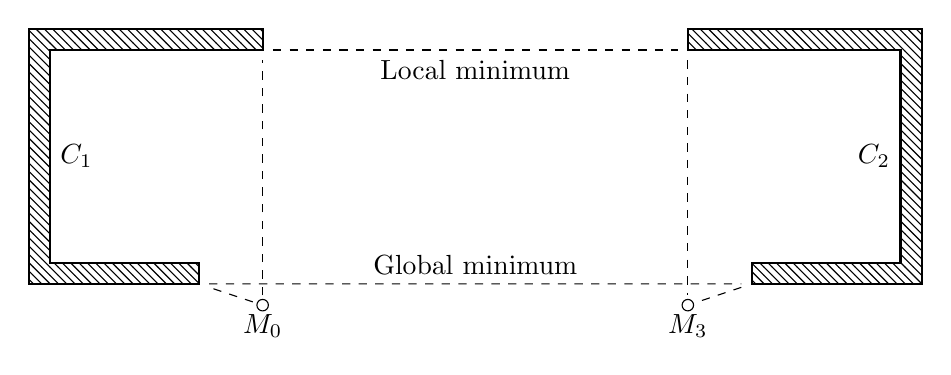
\begin{tikzpicture}[scale=2.7]
    \draw
      (1,-0.2) node(M3){} circle(0.027) node[below] {$M_3$}
      (-1,-0.2) node(M0){} circle(0.027) node[below] {$M_0$};
    \draw [thick,pattern=north west lines]
      (1.3,0) -- (2,0) -- (2,1) node[midway,left]{$C_2$} -- (1,1) node(M2x){} --
      (1, 1.1) -- (2.1,1.1) -- (2.1,-0.1) -- (1.3, -0.1) node(M2) {} --cycle
    % \draw [thick,pattern=north west lines]
      (-1.3,0) -- (-2,0) -- (-2,1) node[midway,right]{$C_1$} -- (-1,1) node(M1x){} --
      (-1, 1.1) -- (-2.1,1.1) -- (-2.1,-0.1) -- (-1.3, -0.1) node(M1){} --cycle;
    \draw[dashed]
      (M0) -- (M1) -- (M2) node[midway,above]{Global minimum} -- (M3);
    \draw[dashed]
      (M0) -- (M1x) -- (M2x) node[midway,below]{Local minimum} -- (M3);
  \end{tikzpicture}
  \end{center}
  \caption{Two tool paths delivering local minimum}
  \label{counter-example}
  \end{figure}
\end{remark}

So,
we consider the following problem,
which has to be solved many times.
Contours consist only of linear segments.
No nested contours.
The order of the contours is fixed.
It is necessary to find a broken line with vertices
on the contours
having the smallest length.

We start from
(arbitrary)
broken line
$L_1$.
We repeat the following process:
for every contour
$C_i$
we find shift its point
$M_i \in C_i$
to that position,
that minimizes the total
length of the broken line,
assuming other points
$M_j$ fixed
($j \ne i$).
This reduces to elementary task
to find a point for which
the sum of the distances to two given points is minimal.

This gives us
the sequence of broken lines
$\{L_k\}$,
The sequence of lengths of these broken lines
decreases monotonously.
Let
$m = \inf |L_k|$
(infium of these lengths),
and
$L_*$ be a polyline with length $m$,
i.e. limit point of the sequence
$\{L_k\}$.
As a metric in the space of broken lines,
one can take the sum of the distances
between vertices with the same indices

\begin{remark}
While applying to real-world problems,
stabilization occurred after a few iterations
(no more than 10),
that is, a broken line
$L_*$ was obtained.
\end{remark}

By construction,
the length of the broken line
$L_*$
cannot be reduced by shifting its vertices individually
or by shifting several vertices,
among which there are no neighbors.

\subsection{Local minimum}

\begin{proposition}
If we move several adjacent vertices of the broken line
$L_*$
so that they remain on the same segments of the contours,
then the length of the resulting broken line will not decrease.
\end{proposition}

\begin{proof}
Consider the shift of two adjacent vertices.
Let four consecutive vertices of the broken line
$L_*$
be located at the points
$M_{i-1}, M_i, M_{i+1}, M_{i+2}$.
Let the points
$M_i \in S_i,
M_{i+1} \in S_{i+1}$
belong to linear segments
of rescpective contours
$S_i \subset C_i,
S_{i+1} \subset C_{i+1}$.
Let us prove
$
\forall M'_i \in S_i,
M'_{i+1} \in S_{i+1}
$:
$
|M_{i-1} M'_i M'_{i+1} M_{i+2}|
\ge
|M_{i-1} M_i M_{i+1} M_{i+2}|
$.

For arbitrary
$M'_i \in S_i$:
$|M_{i-1} M'_i M_{i+1} M_{i+2}|$
is minimal when $M'_i=M_i$,
and
for arbitrary
$M'_{i+1} \in S_{i+1}$:
$|M_{i-1} M_i M'_{i+1} M_{i+2}|$
is minimal when $M'_{i+1}=M_{i+1}$.

Suppose
$
\exists M'_i \in S_i,
\exists M'_{i+1} \in S_{i+1}
$:
$
|M_{i-1} M'_i M'_{i+1} M_{i+2}|
<
|M_{i-1} M_i M_{i+1} M_{i+2}|
$.
It's clear that
$
M'_i \ne M_i,
M'_{i+1} \ne M_{i+1}
$.

Let
$
M_i(s)=M_i+s \cdot \overrightarrow{M_i M'_i}
$,
$
 M_{i+1}(t)= M_{i+1}+t \cdot \overrightarrow{M_{i+1} M'_{i+1}}
$
($s,t \in[0,1]$),
$f(s,t)=
|M_{i-1} M_i(s) M_{i+1}(t) M_{i+2}|
$.

Due to positions of
$M_i$ and $M_{i+1}$:
\begin{equation}
\frac{\partial f(s,t)}{\partial s} \Big|_{(0,0)} \ge 0,
\frac{\partial f(s,t)}{\partial t} \Big|_{(0,0)} \ge 0
\label{partials}
\end{equation}
If,
for instance
$\partial f(s,t) / \partial s \big|_{(0,0)} = 0$,
that is possible only
when
points
$M_{i-1}, M_i, M_{i+1}$
lie on a straight line
(when $M_{i-1}$ and $M_{i+1}$
are on both sides of
$S_i$;
otherwise,
one can replace
$M_{i-1}$ with its reflection
relative to
$S_i$).
So, when both
$$
\frac{\partial f(s,t)}{\partial s} \Big|_{(0,0)}
= 0 =
\frac{\partial f(s,t)}{\partial t} \Big|_{(0,0)}
$$
that means that all four points
$M_{i-1}, M_i, M_{i+1}, M_{i+2}$
lie on the same line
and the broken line is already
the shortest one.

Now,
suppose
at least one derivative in
(\ref{partials})
is not equal to zero.
Consider
$\varphi(t)=f(t,t)$.

$$
\frac{d\varphi}{dt} \Big|_0 =
\frac{\partial f(s,t)}{\partial s} \Big|_{(0,0)}
+
\frac{\partial f(s,t)}{\partial t} \Big|_{(0,0)}
>0
$$

That means
$\exists \tau^* \in [0,1]$:
$\varphi(\tau^*) > \varphi(0)$.
But we assumed
$\varphi(1)<\varphi(0)$,
i.e.
$\varphi(0)<\varphi(\tau^*)>\varphi(1)$.

But note also
that
$\varphi(t)$ is a sum of three terms of a form
$\sqrt{(a+b\cdot t)^2 + (c+d \cdot t)^2}$,
all having positive second derivative,
so
$d^2\varphi(t)/dt^2 \ge 0$,
function
$\varphi(t)$ is convex at
$[0,1]$
and cannot take the value
in the inner point of interval
that is greater than its values
at the ends.

This makes our assumption impossible.

The shift of two neighboring vertices is considered. For more vertices, the proof is similar.

So, the broken
$L_*$
delivers a local minimum.
\end{proof}

\subsection{Global minimum}

Now let's give a condition sufficient
for a broken
$L_*$
to deliver a global minimum.

Let
$M_i \in C_i$ --
vertex of of the broken line
$L_*$.
The adjacent vertices
$M_{i-1}$
and
$M_{i+1}$
are outside
$C_i$,
since there are no nested contours.
By construction of
$L_*$:
$\forall M'_i \in C_i:
|M_{i-1} M_i|+|M_i M_{i+1}|
\le
|M_{i-1} M'_i|+|M'_i M_{i+1}|
$.

\begin{condition}
  \thlabel{cond2}
Let \textbf{one} of the following requirements be satisfied:
\begin{enumerate}
  \item
  Segment $M_{i-1} M_{i+1}$ intersects the contour
  $C_i$,
  i.e.
  $M_i \in M_{i-1} M_{i+1}$
  \item
  The tangent at
  $M_i$
  to the ellipse with foci
  $M_{i-1}$
  and
  $M_{i+1}$
  and passing through
  $M_i$
  separates the ellipse and the contour
  $C_i$.
\end{enumerate}
\end{condition}

\begin{proposition}
  Let \thref{cond2}
  is satisfied for
  (every contour of)
  $L_*$.

  If we move several adjacent vertices of the broken line
  $L_*$ so that they remain on the contours,
  then the length of the resulting broken line does not decrease,
  that is, the broken line
  $L_*$ delivers a global minimum.
\end{proposition}

\begin{proof}
Use the same notations:
consider four adjacent vertices
$M_{i-1}, M_i, M_{i+1}, M_{i+2} \in L_*$.
$M_i \in  C_i,
M_{i+1} \in C_{i+1}$.

Suppose
$
\exists M'_i \in C_i,
\exists M'_{i+1} \in C_{i+1}
$:
$
|M_{i-1} M'_i M'_{i+1} M_{i+2}|
<
|M_{i-1} M_i M_{i+1} M_{i+2}|
$.
Again,
$
M'_i \ne M_i,
M'_{i+1} \ne M_{i+1}
$.

Let
$
M_i(s)=M_i+s \cdot \overrightarrow{M_i M'_i}
$,
$
 M_{i+1}(t)= M_{i+1}+t \cdot \overrightarrow{M_{i+1} M'_{i+1}}
$
($s,t \in[0,1]$),
$f(s,t)=
|M_{i-1} M_i(s) M_{i+1}(t) M_{i+2}|
$.

Now,
\thref{cond2}
gurantees that
$f(s,0)\ge f(0,0)$
for
$s\in[0,1]$,
i.e. again
\begin{equation}
  \frac{\partial f(s,t)}{\partial s} \Big|_{(0,0)} \ge 0,
  \frac{\partial f(s,t)}{\partial t} \Big|_{(0,0)} \ge 0
  % \label{partials}
\end{equation}
This allows us to repeat the rest of the previous proof verbatim.
\end{proof}

\begin{remark}
Suppose that besides the trajectory
$L_*$ ,
there is another trajectory delivering a global minimum.
Then it follows from the proof
that they coincide as lines,
that is,
the difference can only be at
the points of intersection with the contours.
\end{remark}

\thref{cond2}
is easily verified programmatically,
but it can be simplified
so that in most practical cases
to be checked simply visually.

\begin{condition}
When segment
$M_{i-1} M_{i+1}$
doesn't intersects the contour
$C_i$ but
\begin{enumerate}
  \item
  If the vertex
  $M_i$
  is the internal point of the linear segment of the contour
  and the entire contour
  $C_i$
  is on one side of the that segment line
  (which is the tangent from \thref{cond2};
  otherwise there must be a better
  $M'_i\in C_i$).
  \item
  If the vertex
  $M_i$ is terminal
  (belongs to two linear segments of the contour;
  is also vertex of $C_i$),
  and the entire contour is inside
  the corner with the rays from the point
  $M_i$ along these segments.
  \item
  If the region
  $\tilde{C_i}$
  bounded by the contour
  $C_i$ is convex
\end{enumerate}
\end{condition}

\section{Numerical experiments}

The quality assessment of the solutions
of the described algorithm was carried out on several
cutting plans containing real parts.
As a comparison base, we used an algorithm
(see \cite{bi15})
for solving the GTSP problem, which gives an exact solution for the number of contours
$N <33$.

Fig. \ref{gtsp-path} shows the exact solution,
possible positions of the pierce points are visible.
Fig. \ref{ccp-path} shows the solution to the CCP problem
for the same cutting plan.

\begin{figure}
  \begin{center}
    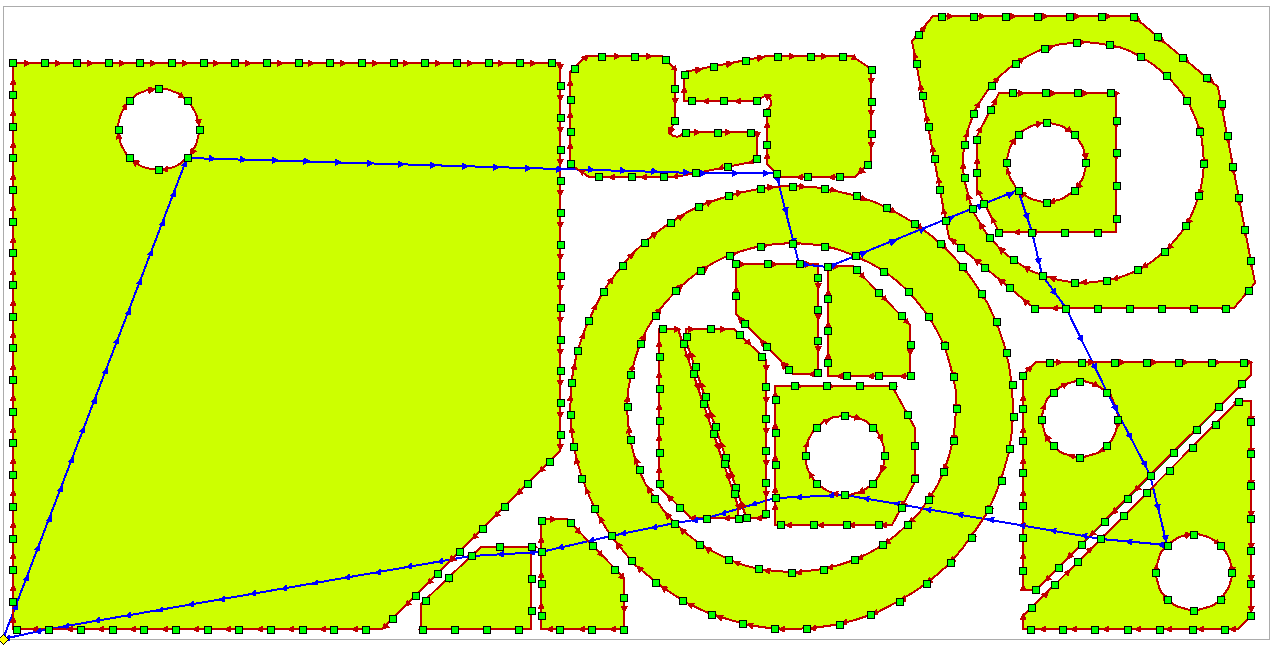
\includegraphics[width=0.95\textwidth]{464-gtsp.png}
  \end{center}
  \caption{Exact solution of GTSP, Job \#464}
  \label{gtsp-path}
\end{figure}

\begin{figure}
  \begin{center}
    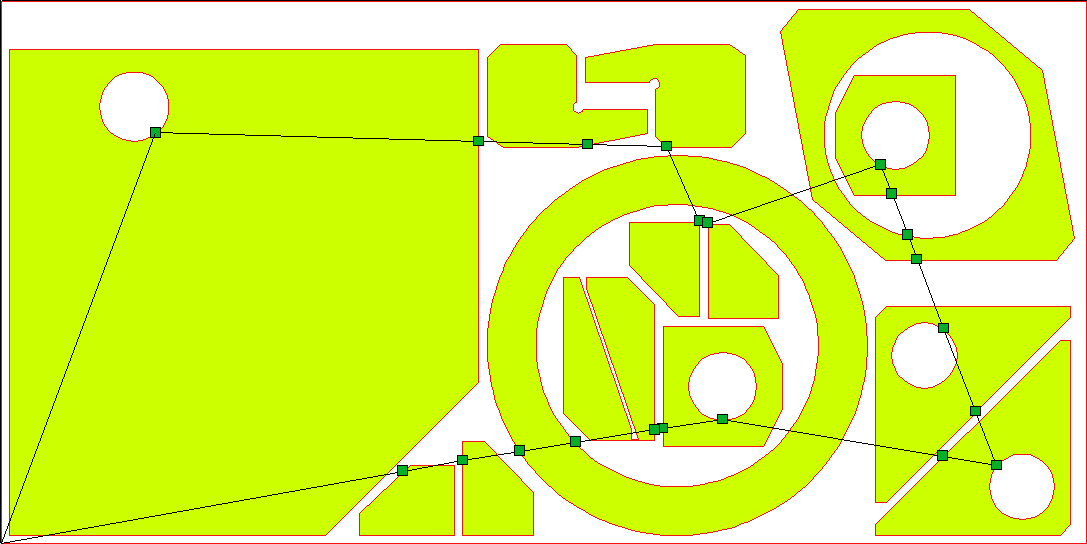
\includegraphics[width=0.95\textwidth]{464-ccp.png}
  \end{center}
  \caption{Solution of CCP, Job \#464}
  \label{ccp-path}
\end{figure}

It can be seen that both algorithms
genererated almost identical routes.
The main difference is caused by the discretization process
to obtain the GTSP task.
Because of this,
the segments of the route that are straight in the CCP solution
turn out to be slightly broken in the GTSP solution,
hence total air move length is slightly larger.
Numerically, this is shown in table \ref{ccp-vs-gtsp}
for several cutting plans.

\begin{table}[h]
  \begin{center}
  \begin{tabular}{l|*{3}{r}}
      Job & \#229 & \#464 & \#3211 \\
      \hline
      \# of parts & 11 & 14 & 17\\
      \# of contours & 12 & 21 & 22 \\
      Parts perimeter, m & 24.609 & 21.717 & 25.051 \\
      \# of GTSP points & 491 & 429 & 493 \\
      $\mathcal L_{GTSP}$, m & 7.729 & 4.743 & 4.557 \\
      $\mathcal L_{CCP}$, m & 7.727 & 4.706 & 4.536 \\
  \end{tabular}
  \caption{Solution quality comparison}
  \label{ccp-vs-gtsp}
  \end{center}
\end{table}

\section{Conclusion}

\begin{enumerate}
  \item
  The problem of minimizing the air move tool of CNC sheet cutting machines
  for the routing problem from the CCP class
  is shown to be reduced
  to a problem without precedence constraint,
  which reduces the number of contours and the operating time of the algorithm
  \item
  A heuristic algorithm for solving the CCP problem is proposed that does not use contour discretization.
  \item
  For any fixed contour visit order,
  an effective algorithm for obtaining a local extremum is developed
  and the conditions under which
  this local minimue is a global one.
  are described.
\end{enumerate}

The direction of further research is the development of the algorithm
for the general case where the pierce points lie
outside the contours
according to the technological requirements of sheet cutting.

\section*{Funding}

This work was supported by the
Russian Foundation for Basic Research
under Grant
20-08-00873.

\bibliographystyle{tfs}
\bibliography{ccp}
\nocite{*}

\end{document}
